\documentclass[12pt]{article}
\usepackage{amsmath,amssymb,mathtools, amsthm}
\usepackage{bbm}
\usepackage{caption}
\usepackage{algorithmic}
\newcommand{\Prob}{\mathbb{P}}
\newcommand{\E}{\mathbb{E}}
\newcommand{\EI}{\mathrm{EI}}
\newcommand{\Dir}{\mathrm{Dirichlet}}
\newcommand{\PI}{\text{P}^*}
\newcommand{\mb}{\mathbf}
\newtheorem{thm}{Theorem}
\newtheorem{algo}{Algorithm}

\title{Bayesian Active Learning for Finding Maximally-valued Exemplars}
\date{\today}
\author{Jialei Wang\thanks{School of Operations Research \& Information Engineering, Cornell University} \and 
Pu Yang\footnotemark[1] \and
Peter I. Frazier\footnotemark[1] \and
}
\begin{document}
\maketitle

\section{Abstract}
We consider a Bayesian optimal search problem, related to active learning and arising in an application to materials science. In active learning, we have training data with unknown binary labels. Obtaining labels is expensive, and we wish to obtain a small number of labels, so that the statistical classifier built from them is good. We consider a variant in which each datapoint has an associated known value, and our goal is to find a datapoint with a positive label and large value.

\section{Introduction}
In many optimal search problems, we need to effectively collect information so as to make the best decisions under uncertainty. In this setting, we need to trade off the reward by sampling (i.e. exploitation) and the cost by aquiring this information (i.e. exploration). For example, in drug discovery, we need to search for a chemical derivative of the base molecule that best treats disease. To achive the goal, we choose molecules to test  to maximize the expected quality of the best compound discovered \cite{Negoescu2010}. Since the budget for testing is limited, we need to test the most informative and high quality molecules. To address this problem, Jones \& Schonlau proposed Expected Improvement algorithm to sample points sequentially \cite{Jones1998} . Ginsbourger used constant liar heuristic to extend Expected Improvement algorithm to parallel setting \cite{Ginsbourger2008} . There are quite a few papers about parallel sampling in active learning research community \cite{Chen2013, Hoi2006, Hoi2006a} , but they only aim to maximize information gain (i.e. pure exploration). In this paper, we consider an optimal search problem in parallel setting, and propose search algorithm using greedy heuristic. We also prove that, our greedy algorithm has a guarantee of performace compared with the optimal solution.

\section{Problem Statement and Application}
We first describe the application that motivates our research, and then we provide mathematical formalism to address a more general problem. In the last sub-section we derive our method in solving this problem.

\subsection{Motivating application}\label{sec: motivate app}
We have two enzymes (Sfp from {\it Bacillus subtilis}, and PaAcpH from {\it Pseudomonas aeruginosa}), and a collection of peptides that can potentially act as a substrate for one or both of these enzymes.  Our goal is to find a peptide that acts as a substrate for both of these enzymes, and is as short as possible.

To support this goal, we can do lab experiments, in which we synthesize a peptide and test, for each enzyme, whether it is a substrate or not.  We need to find a policy that suggests which peptide to synthesize and test next, so as to reach our goal with as few experiments as possible.

Experiments have parallel setup, thus can be done with a batch of peptides at a time, and so the algorithm suggests a batch of peptides at a time, waiting for the results from the experiment before suggesting the next batch of peptides.
A large collection of peptides would be considered by the algorithm for potential synthesis and testing, e.g., all peptides with length less than a given threshold.  That is, we would consider more peptides than just those that are sub-peptides of peptides from the literature known to be substrates for one enzyme.

\subsection{General Problem Statement} \label{sec:prob state}
We now formalize and generalize our problem as an active learning problem, which includes but is not limited to our motivating application.

Let $E$ be a generic search space of exemplars.  In our motivating application, $E$ is the space of peptides.
Each element $x \in E$ has an unknown binary label $y(x)=\{0,1\}$.  A known deterministic function $f(x)$ measures the cost or disutility associated with $x$. Our goal is to perform experiments so as to find $x$ such that it has positive label and its cost function $f(x)$ is minimum.

To obtain labels of exemplars, we can do a batch of experiments, which evaluate a subset $S \subseteq E$ and obtain labels at each time. We measure quality of $S$ by
\begin{equation} \label{eq:fS}
f^*(S)= \begin{dcases}
 \underset{x \in S:y(x)=1}{\min} f(x), & \text{if \,} \{x \in S:y(x)=1\} \neq \emptyset, \\
 \infty,  & \text{if \,} \{x \in S:y(x)=1\} = \emptyset.
 \end{dcases}
\end{equation}

%Let $E$ be any set. For each element $x\in E$, we define a function $f(x)$ that measures the quality of $x$. Larger or smaller values of $f(x)$ may be favored depending on different problem settings. From now on, we assume, without losing generality that smaller values of $f(x)$ are preferred, and for any subset $S\subseteq E$, we measure the quality of $S$ as:
%
%\begin{equation*}
%f^*(S) = \min_{x\in S:\mathbf{h}(x)=0}f(x)
%\end{equation*}
%
%where $\mathbf{h}(x)=(h_1(x),\cdots,h_m(x))$ is a set of constraints that define a subset of "effective elements". We wish to find $S\subseteq E$ with $f^*(S)$ as small as possible, while $S$ it self must satisfy some constraints. A typical constraint is the cardinality of $S$, we usually prefer smaller sets. Other constraints can be applied in different problems.

Let $b$ be a target value and we wish to find $S\subseteq E$ such that $f^*(S)$ is, in some sense, better than $b$. Specifically, we consider the following two measures:
\begin{equation} \label{eq:twomeasure}
\begin{aligned}
&\text{Probability of Improvement: }&\PI(S) = \mathbb{P}(f^*(S) < b)\\
&\text{Expected Improvement: }&\EI(S) = \E [(b-f^*(S))^+]
\end{aligned}
\end{equation}
We wish to find $S$ that maximize one of these two measures. Let $g(S)$ be either $\PI(S)$ or $\EI(S)$ and let the cardinality of $S$ be the only constraint on $S$. Our goal is then:

\begin{equation} \label{eq:opt}
\max_{S\subseteq E:|S|<k}g(S)
\end{equation}

\section{Solution Method}
%If $g(S)$ is $\EI(S)$, from equation \eqref{eq:twomeasure} \eqref{eq:opt}, our goal becomes
%\begin{equation} \label{eq:maxEI}
%\underset{S \subseteq E:|S| \leq k}{\max} \E \left[ (b-f^*(S))^+ \right]
%\end{equation}
%We first prove that the objective function is submodular, and then describe our greedy approach to solve \eqref{eq:maxEI}, finally we show that we have guarantee for our greedy policy compared with optimal policy.
We solve \eqref{eq:opt} using greedy heuristic, that is, starting with empty set $S=\emptyset$, find element $e = \mathrm{arg}\max_e g(S \cup \{e\})-g(S)$ to include in $S$ iteratively until $|S|=K$ for some chosen K. We show first the solution using greedy heuristic has a lower bound, and then present our method.
\subsection{Lower bound of greedy algorithm}
We claim that if objective function is probability of improvement (i.e $\PI(S)$) or expected improvement (i.e $\EI(S)$), the greedy algorithm is guaranteed to achieve a factor $(1-1/e) (\approx 63\%)$ of the optimal value. This lower bound is obtained from a theorem stated in the following:

\begin{thm} \cite{Company1978}
If $F(S)$ is submodular, nondecreasing and $F(\emptyset)=0$, the greedy heuristic always produces a solution whose value is at least $1-[(K-1)/K]^K$ times the optimal value, where $|S| \leq K$. This bound can be achieved for each $K$ and has a limiting value of $1-1/e$, where $e$ is the base of the natural logarithm.
\end{thm}

If we can show our objective functions meet condition in Theorem 1, we find lower bound of the greedy solution.

\begin{thm} 
Probability of improvement $\PI(S)$ is submodular, nondecreasing and $\PI(\emptyset)=0$.
\end{thm}
\begin{proof}
\begin{itemize}
\item
$\PI(\emptyset) = \mathbb{P}(f^*(\emptyset)<b) = \mathbb{P}(\infty<b)=0$.
\item
Suppose $A \subseteq B \subseteq E$ where $E$ is a finite set.
\begin{align*}
\PI(B) &= \mathbb{P}(f^*(B)<b) \\
       &= \mathbb{P}(f^*(B)<b |f^*(A) \geq b) \mathbb{P}(f^*(A) \geq b) + \mathbb{P}(f^*(B)<b |f^*(A)<b) \mathbb{P}(f^*(A)<b) \\
       &= \mathbb{P}(f^*(B)<b |f^*(A) \geq b) \mathbb{P}(f^*(A) \geq b) + \mathbb{P}(f^*(A)<b) \\
       &\geq \mathbb{P}(f^*(A)<b) \\
       &= \PI(A)
\end{align*}
\item
For $e \in E\backslash B$,
\begin{align*}
\PI(A \cup \{e\}) - \PI(A) &= \mathbb{P}(f^*(A \cup \{e\})<b)-\mathbb{P}(f^*(A)<b)\\
                           &= \mathbb{P}(f^*(A \cup \{e\})<b|f^*(A)<b)\mathbb{P}(f^*(A)<b) + \\
                           &\mathbb{P}(f^*(A \cup \{e\})<b|f^*(A)\geq b)\mathbb{P}(f^*(A)\geq b) -\mathbb{P}(f^*(A)<b) \\
                           &=\mathbb{P}(f^*(A)<b) + \mathbb{P}(f^*(A \cup \{e\})<b|f^*(A)\geq b)\mathbb{P}(f^*(A)\geq b) -\\
                           &\mathbb{P}(f^*(A)<b)\\
                           &= \mathbb{P}(f^*(A \cup \{e\})<b|f^*(A)\geq b)\mathbb{P}(f^*(A)\geq b) \\
                           &= \mathbb{P}(f(e)<b, y(e)=1|f^*(A)\geq b)\mathbb{P}(f^*(A)\geq b) \\
                           &= \mathbb{P}(f(e)<b, y(e)=1,f^*(A)\geq b)
\end{align*}
Using similar argument,
\begin{align*}
\PI(B \cup \{e\}) - \PI(B) &= \mathbb{P}(f(e)<b, y(e)=1,f^*(B)\geq b) \\
                           &= \mathbb{P}(f(e)<b, y(e)=1,f^*(A)\geq b, f^*(B\backslash A) \geq b )
\end{align*}
Therefore, $\PI(A \cup \{e\}) - \PI(A) \geq \PI(B \cup \{e\}) - \PI(B)$, thus we conclude that $\PI(S)$ is submodular.
\end{itemize}
\end{proof}

\begin{thm}
Expected improvement $\EI(S)$ is submodular, nondecreasing and $\EI(\emptyset)=0$.
\end{thm}
\begin{proof}
\begin{itemize}
\item
$\EI(\emptyset) = \E[(b-f^*(\emptyset))^+] = \E[0] = 0$.
\item
Suppose $A \subseteq B \subseteq E$ where $E$ is a finite set. Since $f^*(B) \leq f^*(A)$, $b-f^*(B) \geq b-f^*(A)$, and $(b-f^*(B))^+ \geq (b-f^*(A))^+$, therefore, $\E[(b-f^*(B))^+] \geq \E[(b-f^*(A))^+]$.
\item
For $e \in E\backslash B$, consider $\E[(b-f^*(A \cup \{e\}))^+]-\E[(b-f^*(A))^+]$. We can write
\begin{equation*}
(b-f^*(A \cup \{e\}))^+ = \begin{dcases}
                         (b-f^*(A))^+ & \text{if $y(e)=0$} \\
                         (b-\min\{f(e),f^*(A)\})^+ & \text{if $y(e)=1$}
                         \end{dcases}
\end{equation*}
Then 
\begin{align*}
&\E[(b-f^*(A \cup \{e\}))^+]-\E[(b-f^*(A))^+] \\
&= \mathbb{P}(y(e)=1) \E[(b-\min\{f(e),f^*(A)\})^+ -(b-f^*(A))^+|y(e)=1]\\
&= \mathbb{P}(y(e)=1) \mathbb{P}(f(e)<f^*(A)|y(e)=1) \E[(b-e)^+-(b-f^*(A))^+|y(e)=1, f(e)<f^*(A)]\\
&= \E[ \mathbbm{1}_{y(e)=1, f(e)<f^*(A)} ((b-e)^+-(b-f^*(A))^+)]
\end{align*}
Since $f^*(A) \geq f^*(B)$, $\mathbbm{1}_{y(e)=1, f(e)<f^*(A)} ((b-e)^+-(b-f^*(A))^+)) \geq \mathbbm{1}_{y(e)=1, f(e)<f^*(B)} ((b-e)^+-(b-f^*(B))^+))$, thus
\begin{equation*}
\EI(A\cup \{e\})-\EI(A) \geq \EI(B\cup \{e\})-\EI(B)
\end{equation*}
$\EI(S)$ is submodular.

\end{itemize}
\end{proof}



\subsection{Greedy Algorithm}
Suppose we have chosen $S=\{x_1, x_2, \ldots, x_n\}$ as a batch of points we are going to evaluate next, and if we want to incorporate one more point $e$, which is distinct from $x_1, x_2, \ldots, x_n$, such that the objective function increases most, we use the following criterion to find $e$:
\begin{equation} \label{eq:greedy}
\underset{e \in E \backslash S}{\mathrm{arg}\max} \,g(S \cup \{e\})
\end{equation}

\subsubsection{Probability of Improvement}
In the case that objective function is $\PI$, we rewrite \eqref{eq:greedy} as 
\begin{equation} \label{eq:PI}
\underset{e \in E \backslash S}{\mathrm{arg}\max} \,\PI (S \cup \{e\}).
\end{equation} 
Since
\begin{align*}
\PI(S \cup \{e\}) &= \mathbb{P}(f^*(S\cup \{e\})<b)\\
                  &= \mathbb{P}(f^*(S)<b) + \mathbb{P}(f^*(S)\geq b) \mathbb{P}(f(e)<b, y(e)=1|f^*(S)\geq b),
\end{align*}
we can rewrite \eqref{eq:PI} as
\begin{equation} \label{eq:PI2}
\underset{e \in E \backslash S}{\mathrm{arg}\max} \, \mathbb{P}(f(e)<b, y(e)=1|f^*(S)\geq b).
\end{equation}
Thus we use \eqref{eq:PI2} as search criterion for our greedy approach. Note that when $f(e) \geq b$, $\mathbb{P}(f(e)<b, y(e)=1|f^*(S)\geq b)=0$, thus our algorithm will always propose $e$ such that $f(e)<b$. Therefore, it is reasonable to assume that $f(x)<b$ for $\forall x \in S$, and $f^*(S)\geq b$ means $y(x)=0$ for $\forall x \in S$. Now we can write \eqref{eq:PI2} as 
\begin{equation} \label{eq:PI3}
\underset{e \in E \backslash S, f(e)<b}{\mathrm{arg}\max} \, \mathbb{P}(y(e)=1|y(x)=0, \forall x \in S).
\end{equation}

\subsubsection{Expected Improvement}
If objective function is $\EI$, rewrite \eqref{eq:greedy} as 
\begin{equation} \label{eq:EI}
\underset{e \in E \backslash S}{\mathrm{arg}\max} \, \E \left[ (b-f^*(S \cup \{e\}))^+ \right].
\end{equation}
Since choosing $e$ such that $f(e) \geq b$ has no contribution to the objective function, by using similar argument as dealing with probability of improvement, we argue that $f(x)<b$ for $\forall x \in S$. Thus
\begin{equation*}
f^*(S)  \begin{dcases}
         =\infty & \text{if $y(x)=0$ for $\forall x \in S$},\\
         < b & \text{else}.
 \end{dcases}
\end{equation*}
Now objective function we want to maximize becomes
\begin{align*}
&\E \left[ (b-f^*(S \cup \{e\}))^+ \right] \\
&= \E[(b-f(e))^+ \mathbbm{1}_{f^*(S)=\infty, y(e)=1}]+ \E[ (b-f^*(S \cup \{e\}))^+ \mathbbm{1}_{f^*(S)<b}] \\
&= \E[(b-f(e))^+ \mathbbm{1}_{f^*(S)=\infty, y(e)=1}]+ \E[ (b-f^*(S)) \mathbbm{1}_{f^*(S)<b}] + \E[(f^*(S)-f(e)) \mathbbm{1}_{y(e)=1, f(e)<f^*(S)<b}].
\end{align*}
Equation \eqref{eq:EI} is equivalent to 
\begin{equation} \label{eq:EI2}
\underset{e \in E \backslash S, f(e)<b}{\mathrm{arg}\max} \, \E[(b-f(e)) \mathbbm{1}_{f^*(S)=\infty, y(e)=1}]+\E[(f^*(S)-f(e)) \mathbbm{1}_{y(e)=1, f(e)<f^*(S)<b}].
\end{equation}
For $e \in E \backslash S, f(e)<b$,
\begin{align*}
&\E[(b-f(e)) \mathbbm{1}_{f^*(S)=\infty, y(e)=1}] = (b-f(e)) \mathbb{P}(y(e)=1, y(x)=0, \forall x \in S)\\
&\E[(f^*(S)-f(e)) \mathbbm{1}_{y(e)=1, f(e)<f^*(S)<b}]\\
&=\E[\E[(f^*(S)-f(e)) \mathbbm{1}_{y(e)=1, f(e)<f^*(S)<b}]|f^*(S)=l]\\
&= \sum_{l \in L, f(e)<l} \mathbb{P}(y(e)=1|f^*(S)=l)(l-f(e))\mathbb{P}(f^*(S)=l),\\
\end{align*}
where $L = \{f(x): x \in S\}$. If we rank elements in $S$ such that $f(x_i) \leq f(x_j), \forall i<j, x_i,x_j \in S$, we can write equation above as
\begin{equation*}
\sum_{i=1}^{|S|} \mathbb{P}(y(e)=1, y(x_i)=1, y(x_j)=0, \forall j<i, x_i,x_j \in S)(f(x_i)-f(e))^+
\end{equation*}
Since $\mathbb{P}(y(e)=1, \mathcal{F}(x_1,\ldots,x_{|S|}) \propto \mathbb{P}(y(e)=1| \mathcal{F}(x_1,\ldots,x_{|S|})$, and coefficient is known given $S$, we can write our criterion for greedy algorithm as
\begin{equation} \label{eq:EI3}
\underset{e \in E \backslash S}{\mathrm{arg}\max} \, c_0 \mathbb{P}_0(e)(b-f(e))^+ + \sum_{i=1}^{|S|} c_i \mathbb{P}_i(e)(f(x_i)-f(e))^+,
\end{equation}
where
\begin{align*}
&\mathbb{P}_0(e)=\mathbb{P}(y(e)=1|y(x)=0, \forall x \in S)\\
&\mathbb{P}_i(e)=\mathbb{P}(y(e)=1|y(x_i)=1, y(x_j)=0, \forall j<i, x_i,x_j \in S),
\end{align*}
and $c_i, i=0,\ldots,|S|$ are known coefficients.

%Since
%\begin{equation*}
%(b-f^*(S \cup \{e\}))^+ =      \begin{dcases}
%                    (b- f^*(S))^+ & \text{if $y(e)=1, f(e)<f^*(S)$ ,} \\
%                    (b- \min \{f(e), f^*(S)\})^+      & \text{if $y(e)=1$ ,}
%                    \end{dcases}
%\end{equation*}
%%&= \E [b-f^*(S) + \mathbbm{1}_{\{y(e)=1, f(e) < f^*(S)\}} [f^*(S)-f(e)] ]
%After some algebra we can write \eqref{eq:finde} as
%\begin{align*}
%&\underset{e \in E \backslash S}{\mathrm{arg}\max} \E [ \mathbbm{1}_{\{y(e)=1, f(e) < f^*(S)\}} [f^*(S)-f(e)] ] \\
%%&=\underset{e \in E \backslash S}{\mathrm{arg}\max} \E [ \E [\mathbbm{1}_{\{y(e)=1, f(e) < f^*(S)\}} [f^*(S)-f(e)] | f^*(S)]\\
%%&= \underset{e \in E \backslash S}{\mathrm{arg}\max} \E [ \mathbbm{1}_{\{f(e)<f^*(S)\}} \mathbb{P} (y(e)=1 | f^*(S)) [f^*(S)-f(e)]] \\
%&= \underset{e \in E \backslash S}{\mathrm{arg}\max} \sum_{i=1}^{|S|} \mathbb{P} (y(e)=1, y(x_i)=1, y(x_j)=0, \forall j <i) [f(x_i)-f(e)]^+ \\
%&+ \mathbb{P} (y(e)=1, y(x_j)=0, \forall j) [b-f(e)]^+
%\end{align*}
%where $f(x_i)<=f(x_j)$ for $\forall i<j, x_i,x_j \in S$.
%Since
%\begin{align*}
%&\mathbb{P} (y(e)=1, y(x_i)=1, y(x_j)=0, \forall j <i)\\
%&= \mathbb{P}(y(x_1)=0) \mathbb{P}(y(x_2)=0|y(x_1)=0) \ldots \mathbb{P}(y(e)=1|\mathcal{F}(x_1,x_2,\ldots,x_i)\\
%&\propto \mathbb{P}(y(e)=1|\mathcal{F}(x_1,x_2,\ldots,x_i)
%\end{align*}



\section{Application}
We apply our algorithm to finding minimally-sized peptide substrates. The problem has been described in \ref{sec: motivate app}.

\subsection{Statistical Method}
We use Naive Bayes as the classification method, which, despite the name, has performed quite well in many cases. Let $X=(X_1,\ldots,X_n)$ be an instance with $n$ features and $Y$ be its label. By Bayes's Rule, we have:

\begin{equation*}
\Prob(Y=y|X=x)=\frac{\Prob(X=x|Y=y)\Prob(Y=y)}{\Prob(X=x)}=\frac{\Prob(X=x|Y=y)\Prob(Y=y)}{\sum_{y'}\Prob(X=x|Y=y')\Prob(Y=y')}
\end{equation*}

The Naive Bayes classifier assumes that the presence or absence of a particular feature is unrelated to the presence or absence of any other feature, given the class variable, i.e.

\begin{equation*}
\Prob(Y=y|X=x) = \frac{\prod_{j=1}^n\Prob(X_j=x_j|Y=y)\Prob(Y=y)}{\sum_{y'}\prod_{j=1}^n\Prob(X_j=x_j|Y=y)\Prob(Y=y)}
\end{equation*}

In our motivation application, we have a set of peptides, each with length less than or equal to $L$. Each peptide is a sequence of amino acids. We use a reduced alphabet for amino-acids, i.e., we group them into $K$ groups. For each peptide, let $A_i$ be the amino acid on position $j$, and let $X_i$ be the class of this amino acid. For a specific enzyme, let $Y(x)=1$ if peptide $x$ is a substrate for that enzyme and 0 if not.

We let $\theta_{y,j}(k)=\Prob(X_i=k|Y(X)=y)$, for each $j=1,\ldots,L$, $k=1,\ldots,K$ and $y\in\{0,1\}$. We further assume some known prior distribution $\Prob(Y(x)=y)$, $y\in\{0,1\}$. Let $\theta$ be the full set of parameters $\theta_{y,j}(k)$, for $j=1,\ldots,L$, $k=1,\ldots,K$ and $y\in\{0,1\}$. Then, given an unlabeled peptide, we can calculate its probability being a substrate as:

\begin{equation} \label{eq:model}
  \Prob\left(Y(x) = 1 | \theta\right) =
  \frac{\Prob(Y(x)=1) \prod_{j} \theta_{1,j}(x_j)}{
  \left[ \Prob(Y(x)=1) \prod_{j} \theta_{1,j}(x_j)\right] +
  \left[ \Prob(Y(x)=0) \prod_{j} \theta_{0,j}(x_j)\right]}
\end{equation}

We estimate the parameters $\theta_{y,j}(k)$ using Bayesian inference. We assume for each $j=1,\ldots,L$, $y\in\{0,1\}$, the vector $\theta_{y,j}\sim\Dir(\alpha_{y,j}(1),\ldots,\alpha_{y,j}(K))$. A good initial choice for the parameter vector $\alpha_{y,j} = (\alpha_{y,j}(1),\ldots,\alpha_{y,j}(6))$ can be choosing $\alpha_{y,j}(k)$ to be constant across $k$, and $y$, and to only depend upon $j$. Since amino acids further from the serine are less likely to have a strong influence on its activity, we choose this value to be $1$ in the positions next to the serine and to increase as $j$ moves further.

We further assume two hyper parameters $\gamma_0$ and $\gamma_1$ that characterize the distribution for $y=0$ and $y=1$ respectively. Then, with the prior distribution and hyper parameters, our posterior distribution is also Dirichlet. In particular, it is 
$\Dir( \alpha_{y,j}(1) + \gamma_yN_{y,j}(1), \ldots, \alpha_{y,j}(K) + \gamma_yN_{y,j}(K))$,
where $N_{y,j}(k)$ counts how many peptides $x$ in the training data with $Y(x)=y$ had $x_j=k$.  That is, it counts how many peptides had amino acid $j$ in class $j$.

Since our training data is expensive and highly skewed, we use the leave-one-out cross validation procedure to choose the optimal hyper parameters. For each setting of the hyper parameters, we obtain an receiver operating characteristic(ROC) curve using the result of the leave-one out procedure and choose the setting with highest AUC(area under curve).

%[Put two ROC curves here, one for leave-one-out and one for using the 1st data set as training and 2nd data set as test, to be continued ...]

\begin{figure}[hpt] 
\center
\begin{minipage}[b]{0.45\linewidth}
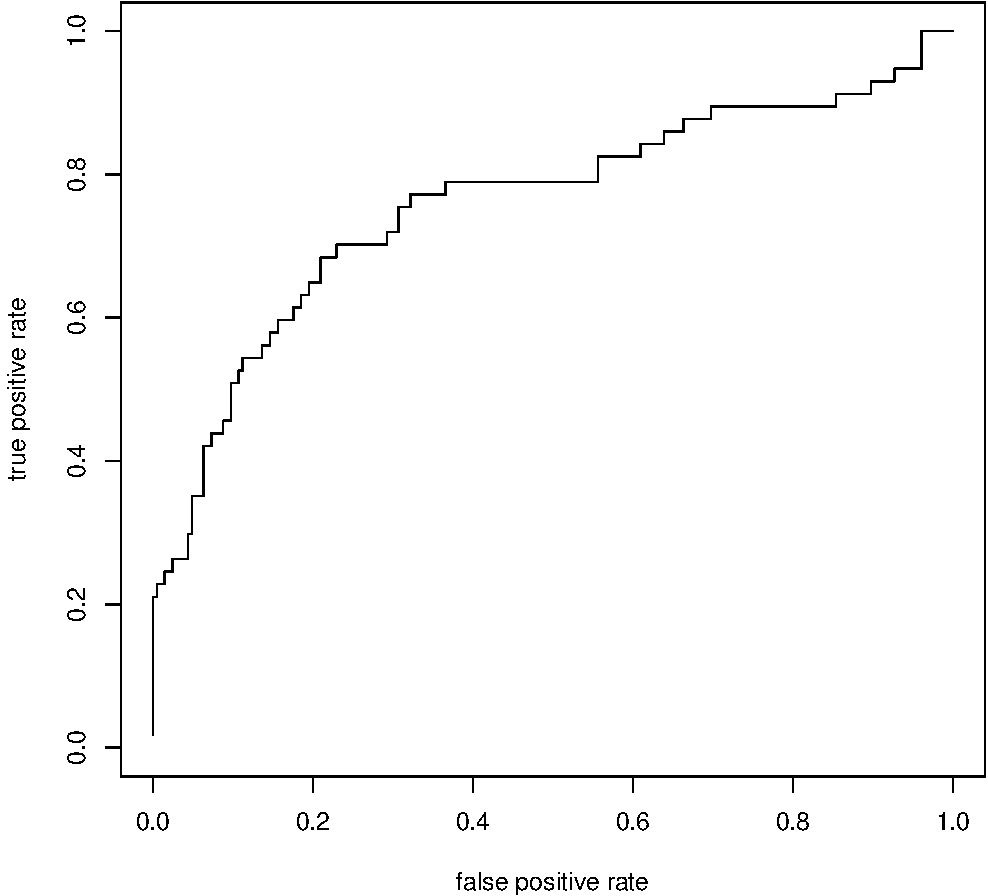
\includegraphics[width=\textwidth]{pic/ROC_DS1_1000_025.pdf}
\caption*{using data set \#0 \& \#1}
\end{minipage}
\begin{minipage}[b]{0.45\linewidth}
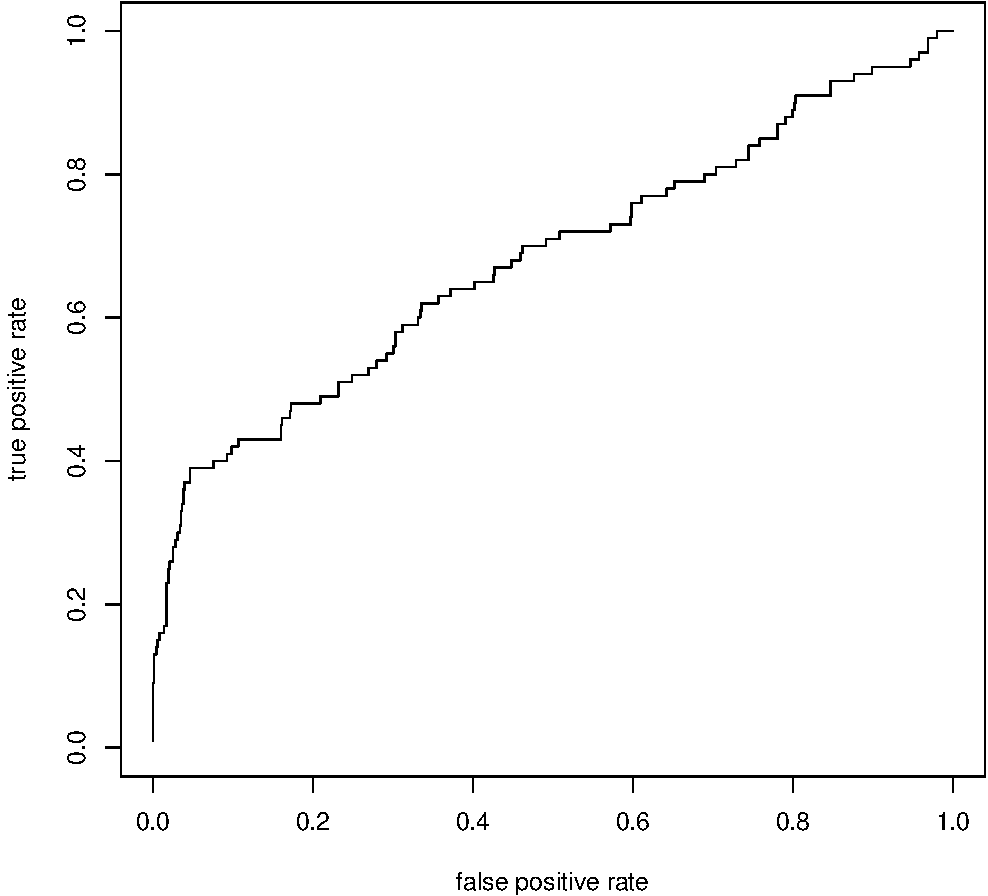
\includegraphics[width=\textwidth]{pic/ROC_DS2_1000_025.pdf}
\caption*{using data set \#0,\#1 \& \#2}
\end{minipage}
\caption{ ROC curve using leave-one-out cross validation}
\label{fig:ROC}
\end{figure}

In Figure \ref{fig:ROC}, note ROC curve to the left is better than the one to the right. This is because data set \#2 was generated by our algorithm based on the previous two data sets, and due to the exploration manner of our algorithm, data set \#2 should lie in the region that is more challenging for the classifier. Thus it is reasonable that our classifer performs worse using all available data sets. 

\subsection{Greedy Algorithm}
\subsubsection{Probability of Improvement}
We use equation \eqref{eq:PI3}, embeded in statistical model described in the previous section, to find peptides to sample next. 

Write equation \eqref{eq:model} as
\begin{equation} \label{model1}
\Prob\left(Y(x) = 1 | \theta\right) =
\frac{\prod_j \eta_j(x_j)}{\prod_j \eta_j(x_j) + \frac{\Prob(Y(x)=0)}{\Prob(Y(x)=1)}},
\end{equation}
where
\begin{equation*}
\eta_j(x_j) = \frac{\theta_{1,j}(x_j)}{\theta_{0,j}(x_j)} \text{\,\,\,for $\forall j \in \{1,\ldots,L\}$}. 
\end{equation*}
Then we can write equation \eqref{eq:PI3} as
\begin{equation} \label{eq:PI4}
\underset{e \in E \backslash S, f(e)<b}{\mathrm{arg}\max} \, \frac{\prod_j \eta_j(e_j)}{\prod_j \eta_j(e_j) + \frac{\Prob(Y(e)=0)}{\Prob(Y(e)=1)}},
\end{equation}
where 
\begin{equation*}
\eta_j(e_j)=\frac{\Prob(e_j|Y(e)=1,Y(x)=0, \forall x \in S)}{\Prob(e_j|Y(e)=0,Y(x)=0, \forall x \in S)}.
\end{equation*}
We can formulate equation \eqref{eq:PI4} as a Mixed-Integer Nonlinear Programming (MINLP),
\begin{equation} \label{eq:PI5}
\begin{align*}
\max \quad &\frac{\prod_j \Sigma_k x_j(k) \eta_j(k)}{\prod_j \Sigma_k x_j(k) \eta_j(k) + \frac{\Prob(Y(x)=0)}{\Prob(Y(x)=1)}} \\
\text{s.t} \quad &k \in \{1,\ldots,K\} \\
&x_j(k) \in \{0,1\}\\
&\Sigma_k x_j(k)=1,
\end{align*}
\end{equation}
where
\begin{equation*}
x_j(k)=\begin{dcases}
        1 & \text{if $e_j=k$}\\
        0 & \text{else}.
\end{dcases}
\end{equation*}
There are quite a few available software packages that can solve equation \eqref{eq:PI5} based on branch-and-bound. This is summarized in Algorithm \ref{algo1}.
\begin{algo}(Probability of Improvement) \label{algo1}\\
\begin{algorithmic}[1]
\REQUIRE Inputs $\text{M, J, K}$, data set D and prior distribution of $\theta_y \sim \text{Dirichlet} (\boldsymbol \alpha_y), y \in \{1,0\}$
\STATE $S \leftarrow \emptyset $
\STATE Calculate posterior distribution of $\theta_1 \sim \text{Dirichlet} (\boldsymbol \alpha_1|\{x|x \in D,y(x)=1\})$.
\FOR{$m=1$ to $M$} 
\STATE COUNT $\leftarrow 0$
\STATE Calculate posterior distribution of $\theta_0 \sim \text{Dirichlet} (\boldsymbol \alpha_0|\{x|x \in D,y(x)=0\} \cup S)$.
\LOOP 
\STATE Sample $\theta_1$ from $\text{Dirichlet} (\boldsymbol \alpha_1|\{x|x \in D,y(x)=1\})$ and $\theta_0$ from $\text{Dirichlet} (\boldsymbol \alpha_0|\{x|x \in D,y(x)=0\} \cup S)$.
\STATE $\eta \leftarrow \frac{\theta_1}{\theta_0}$
\STATE Solve MINLP in equation \eqref{eq:PI5} to find $x$.
\STATE COUNT $\leftarrow$ COUNT $+ x$.
\ENDLOOP
\FOR {$j=1$ to $J$}
\STATE $e_j \leftarrow \underset{k \in \{1,\ldots,K\}}{\mathrm{arg}\max} \, \text{COUNT}_{kj}$
\ENDFOR
\STATE $S \leftarrow (S, e)$
\ENDFOR
\end{algorithmic}
\end{algo}
To see the performance of probability of improvement algorithm, we compare it with two other methods: one method is to pick the most probable peptides based on posterior distribution, and the other is to randomly mutate known peptides $x$ such that $y(x)=1$ as our new recommendations. We use probability that shortest peptide $x$ with $y(x)=1$ has length smaller or equal to 12 as a measure of quality, to do the benchmark, and we show the result in Figure \ref{fig:PI}.
\begin{figure}[hpt] 
\center
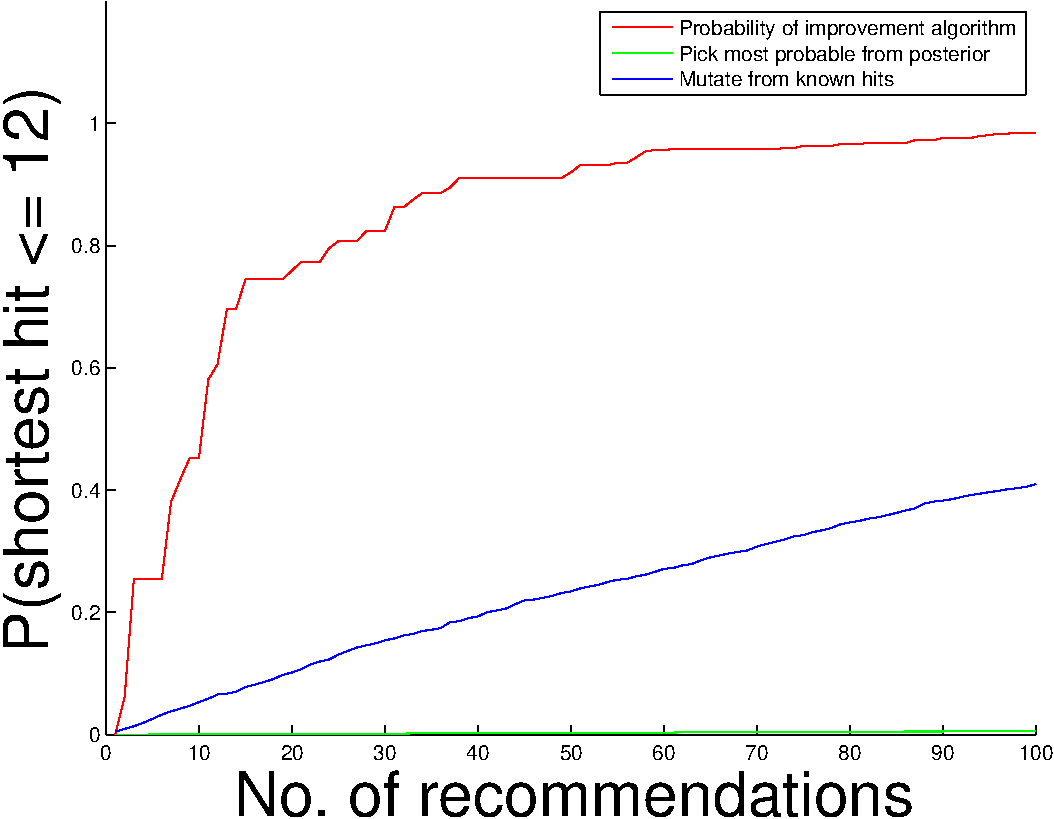
\includegraphics[width=0.6\textwidth]{pic/maxP_comparison.pdf}
\caption{Benchmark of probability of improvement algorithm}
\label{fig:PI}
\end{figure}

\subsubsection{Expected Improvement}
Notice that each term in the summation of Equation \eqref{eq:EI3} has a similar structure as equation \eqref{eq:PI3}. Suppose $S=\{p^1,\ldots,p^{|S|}\}$, then we can write \eqref{eq:EI3} as a MINLP:

\begin{equation} \label{eq:EI4}
\begin{align*}
\max \quad &\Sigma_{i=0}^{|S|} c_i \frac{\prod_j \Sigma_k x_j(k) \eta_j^i(k)}{\prod_j \Sigma_k x_j(k) \eta_j^i(k) + \frac{\Prob(Y(x)=0)}{\Prob(Y(x)=1)}} (f_i-f(e))^+ \\
\text{s.t} \quad &k \in \{1,\ldots,K\} \\
&x_j(k) \in \{0,1\}\\
&\Sigma_k x_j(k)=1,
\end{align*}
\end{equation}
where
\begin{equation*}
x_j(k)=\begin{dcases}
        1 & \text{if $e_j=k$}\\
        0 & \text{else},
\end{dcases}
\end{equation*}
\begin{equation*}
f_i=\begin{dcases}
        b & \text{if $i=0$}\\
        f(p^i)  & \text{else},
\end{dcases}
\end{equation*}
and $c_i$'s are known coefficients. We summarize it in Algorithm \ref{algo2}.

\begin{algo}(Expected Improvement) \label{algo2}\\
\begin{algorithmic}[1]
\REQUIRE Inputs $\text{M, J, K}$, data set D and prior distribution of $\theta_y \sim \text{Dirichlet} (\boldsymbol \alpha_y), y \in \{1,0\}$
\STATE $S \leftarrow \emptyset $
\FOR{$m=1$ to $M$} 
\STATE COUNT $\leftarrow 0$
\IF{$S$ is not empty}
\STATE Sort elements in $S$ as $\{p^1,\ldots,p^{|S|}\}$ such that $f(p^i) \leq f(p^j), \forall i<j$.
\ENDIF
\STATE Calculate posterior distribution of $\theta_1^0 \sim \text{Dirichlet} (\boldsymbol \alpha_1|\{x|x \in D,y(x)=1\})$ and $\theta_0^0 \sim \text{Dirichlet} (\boldsymbol \alpha_0|\{x|x \in D,y(x)=0\} \cup S)$.
\FOR{$i=1$ to $|S|$}
\STATE Calculate posterior distribution of $\theta_1^i \sim \text{Dirichlet} (\boldsymbol \alpha_1|\{x|x \in D,y(x)=1\} \cup \{p^i\})$ and $\theta_0^i \sim \text{Dirichlet} (\boldsymbol \alpha_0|\{x|x \in D,y(x)=0\} \cup \{p^j|j<i\})$.
\ENDFOR
\LOOP 
\STATE Sample $\theta_1^{i=0:|S|}$ and $\theta_0^{i=0:|S|}$ from posterior distribution.
\STATE $\eta^{i=0:|S|} \leftarrow \frac{\theta_1^{i=0:|S|}}{\theta_0^{i=0:|S|}}$
\STATE Solve MINLP in equation \eqref{eq:EI4} to find $x$.
\STATE COUNT $\leftarrow$ COUNT $+ x$.
\ENDLOOP
\FOR {$j=1$ to $J$}
\STATE $e_j \leftarrow \underset{k \in \{1,\ldots,K\}}{\mathrm{arg}\max} \, \text{COUNT}_{kj}$
\ENDFOR
\STATE $S \leftarrow (S, e)$
\ENDFOR
\end{algorithmic}
\end{algo}
Benchmark to be added here.

\section{Conclusion}
We presented two greedy heuristic algorithms solving active learning problem described in \ref{sec:prob state}, and proved that both of these two algorithms guarantee to achieve at least a factor (1-1/e) of the optimal value. From benchmark results, we further showed that these two algorithms outperformed another two heuristic search methods. In addition to theoretic results, We demonstrated effectiveness of our methods by applying them to optimal experimental design problem in material science, in which we are searching for shortest peptides that act as a substrate for some specific enzymes. We developed a Naive Bayes classifier to model the problem, and used our algorithm to propose candidates for testing by experiment. From the preliminary testing result made by our experimental collaborator, we have found a few short peptides that are very likely to be substrate of target enzymes.

\bibliography{UCSD}
\bibliographystyle{apalike}
\end{document}
